\emph{For the following experiments, $\lambda=11$.}\\
\\
Fig. \ref{fig:uaddevolution} below shows the evolution of the value of $J^{*}$ with $U_{add}$.\\
\begin{figure}[h]
	\caption{Evolution of $J^{*}$ with $U^{add}$}
	\label{fig:uaddevolution}
	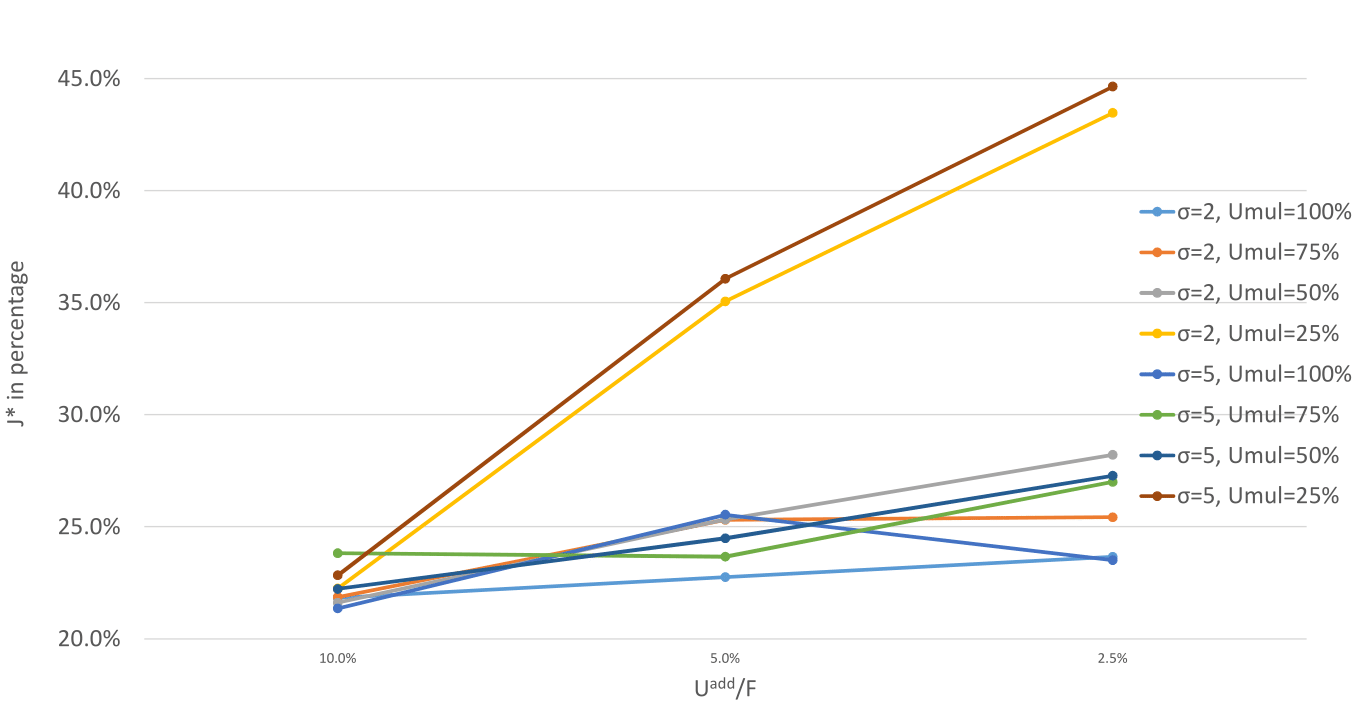
\includegraphics[width=7in]{figures/uadd.png}
\end{figure}
\\
As intuitively guessed, the more uncertainty i.e. freedom to the knobs there is, the smaller $J^{*}$ is.
More precisely, the tendencies observed are the following :\\
\begin{itemize}
	\item The only case where $U^{add}$ drastically changes $J^{*}$ is when it compensates the fact that $U^{mul}$ is very small ($25\% $ in our case). In this situation, $U^{add}$ always gives more freedom to the knobs than $U^{mul}$, and $J^{*}$ improves proportionally to the increase of $U^{add}$. We described this effect in the last paragraph \ref{subsec:umul} and discarded these $U^{mul}$ too small values.\\
However, this is a good way of monitoring the usefulness of $U^{add}$.
	\item For larger $U^{mul}$ values, $U^{add}$ helps diminishing $J^{*}$ value by $2-10 \% $ (depending on the relative importance of $U^{add}$ in comparison to $U^{mul}$), as expected.
\end{itemize}
Below are 3 groups of figures. They display especially, for each of the 3 values of $U^{add}$, how the resulting congestion pattern fitting and the history of the knobs trough the execution evolve with $U^{mul}$ and $\sigma$.
\begin{figure}[!h]
	\centering
	\caption{$\mathbf{\frac{U_{add}}{\widetilde{F}}=2.5\%}$. Congestion pattern matching plots : evolution with $U_{mul}$ and $\sigma$.}
	\label{fig:uaddcp25}
	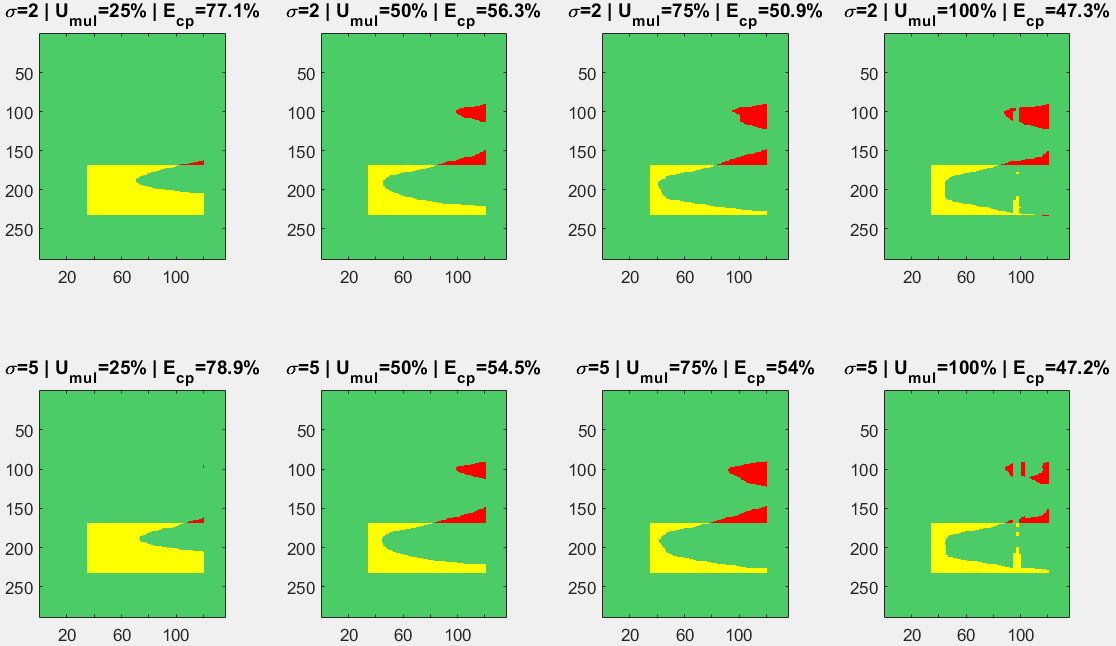
\includegraphics[width=7in]{figures/results_figures/Uadd/cp_Uadd_25_lambda_11.png}
\end{figure}	
\begin{figure}[!h]
\centering
	\caption{$\mathbf{\frac{U_{add}}{\widetilde{F}}=2.5\%}$. [0-10] knobs history plots : evolution with $U_{mul}$ and $\sigma$.}
	\label{fig:uaddknobs25}
	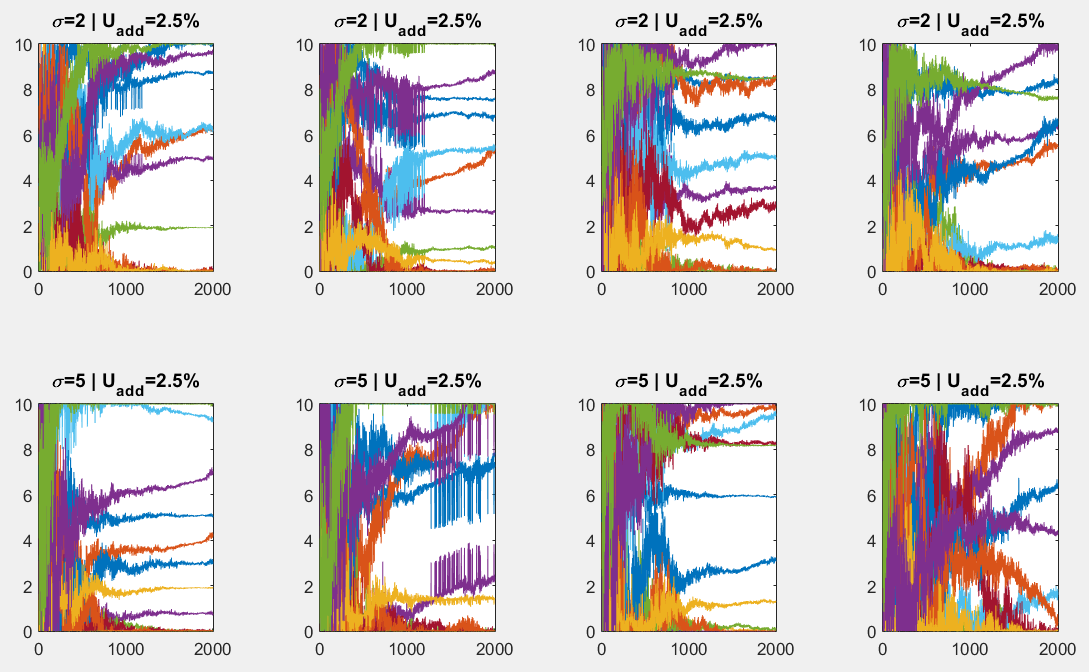
\includegraphics[width=7in]{figures/results_figures/Uadd/knobs_Uadd_25_lambda_11.png}
\end{figure}
\begin{figure}[!h]
	\centering
	\caption{$\mathbf{\frac{U_{add}}{\widetilde{F}}=5\%}$. Congestion pattern matching plots : evolution with $U_{mul}$ and $\sigma$.}
	\label{fig:uaddcp5}
	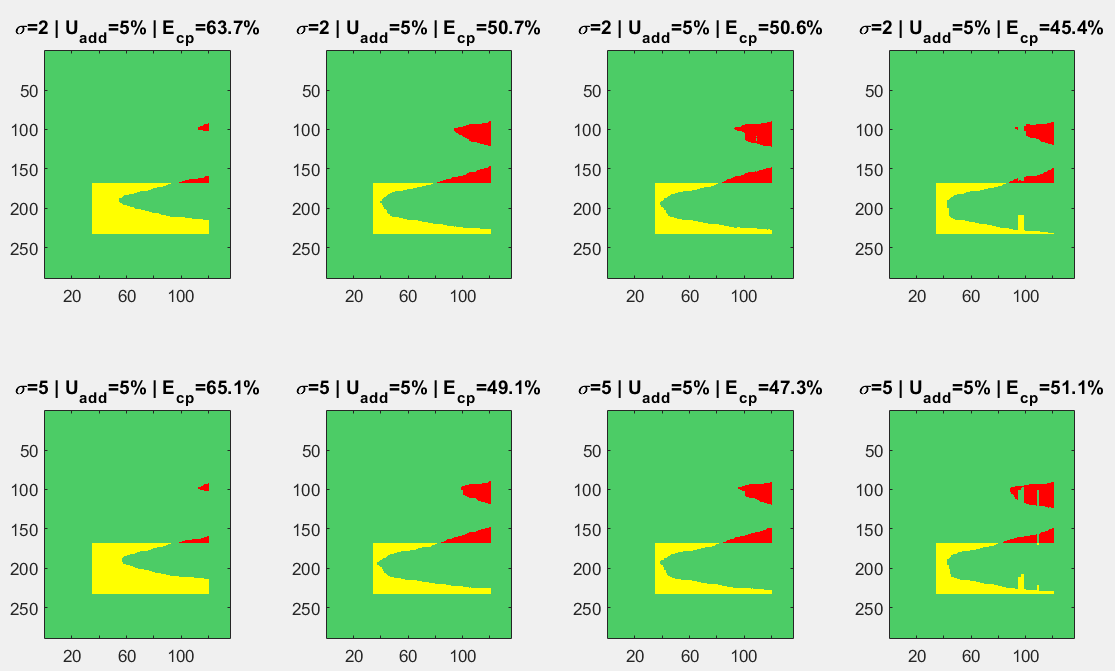
\includegraphics[width=7in]{figures/results_figures/Uadd/cp_Uadd_5_lambda_11.png}
\end{figure}	
\begin{figure}[!h]
	\centering
	\caption{$\mathbf{\frac{U_{add}}{\widetilde{F}}=5\%}$. [0-10] knobs history plots : evolution with $U_{mul}$ and $\sigma$.}
	\label{fig:uaddknobs5}
	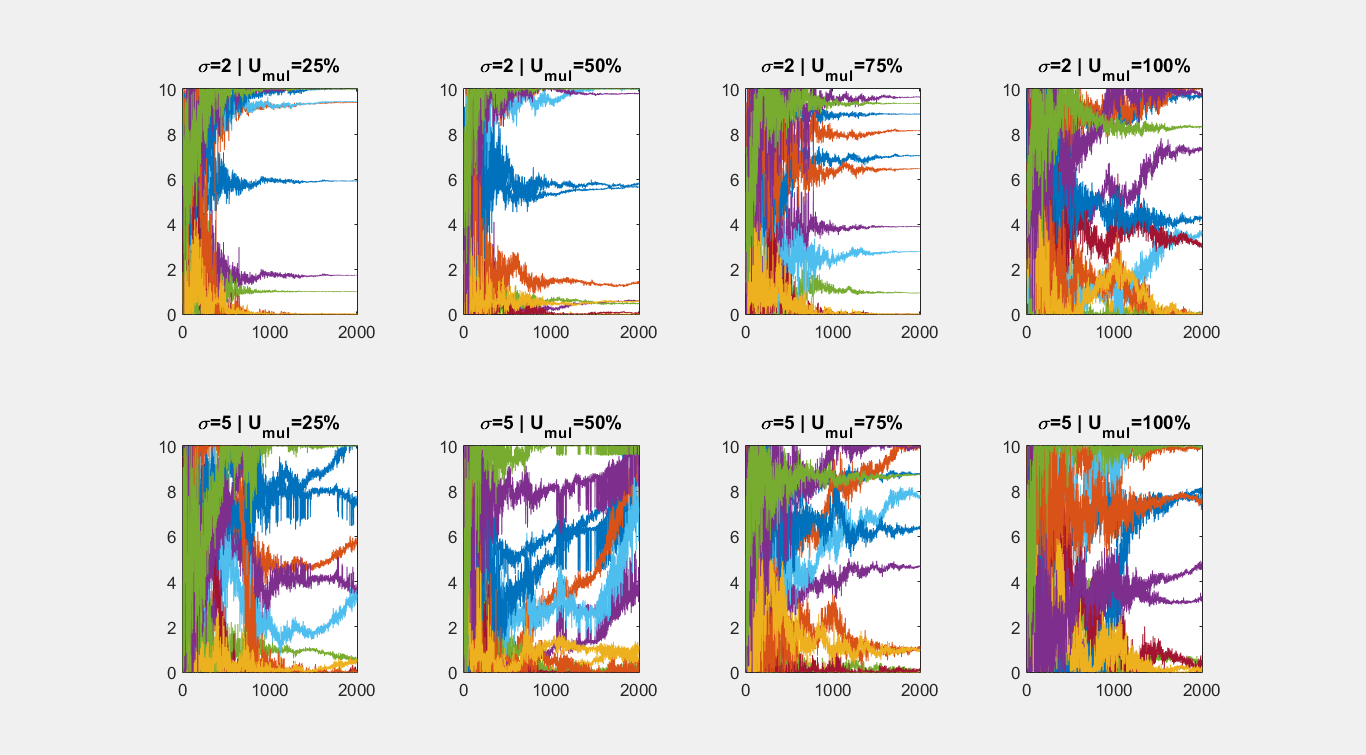
\includegraphics[width=7in]{figures/results_figures/Uadd/knobs_Uadd_5_lambda_11.png}
\end{figure}
\begin{figure}[!h]
	\centering
	\caption{$\mathbf{\frac{U_{add}}{\widetilde{F}}=10\%}$. Congestion pattern matching plots : evolution with $U_{mul}$ and $\sigma$.}
	\label{fig:uaddcp10}
	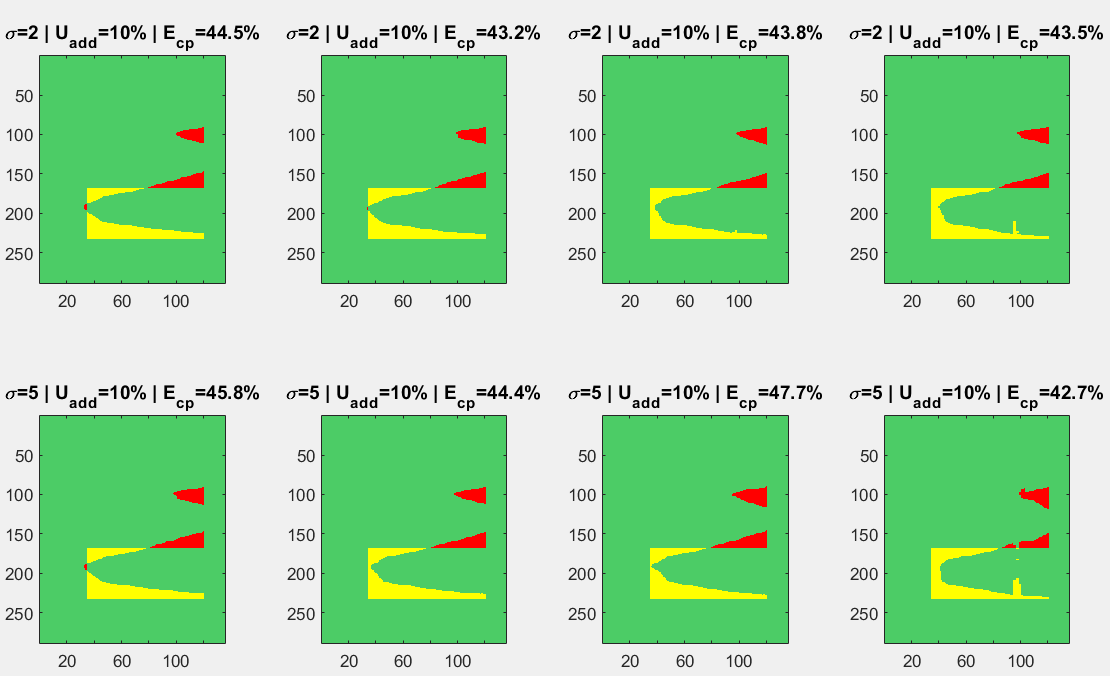
\includegraphics[width=7in]{figures/results_figures/Uadd/cp_Uadd_10_lambda_11.png}
\end{figure}	
\begin{figure}[!h]
	\centering
	\caption{$\mathbf{\frac{U_{add}}{\widetilde{F}}=10\%}$. [0-10] knobs history plots : evolution with $U_{mul}$ and $\sigma$.}
	\label{fig:uaddknobs10}
	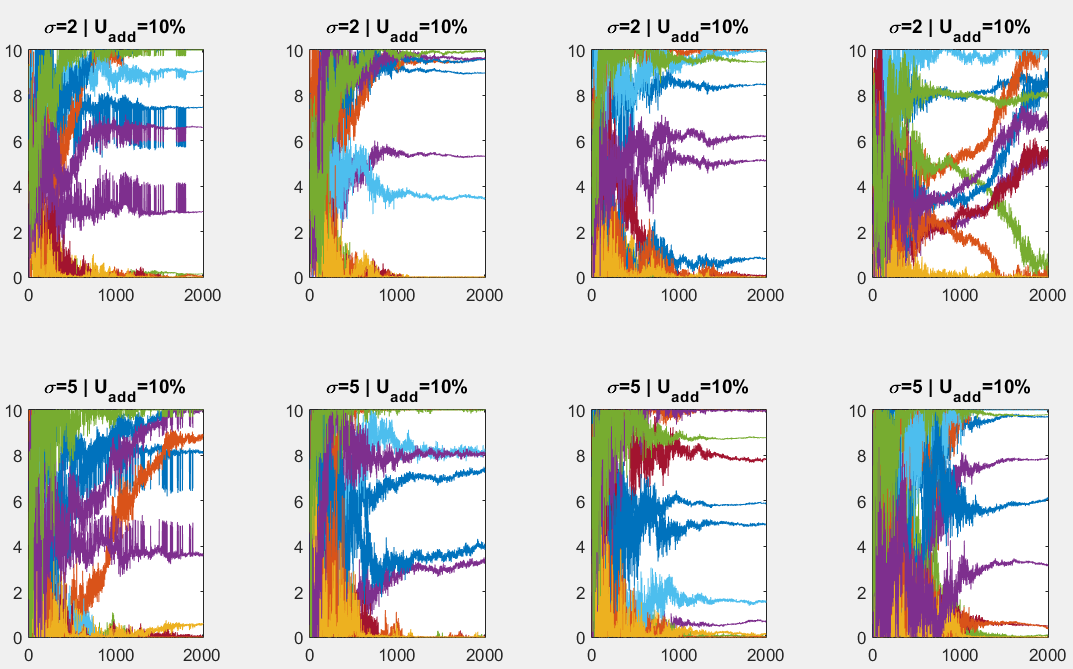
\includegraphics[width=7in]{figures/results_figures/Uadd/knobs_Uadd_10_lambda_11.png}
\end{figure}
\newpage

The $3$ preceding congestion pattern figures show how $U^{add}$ progressively overrides $U^{mul}$: with $U^{add}=2.5\% $, the resulting congestion shape is very dependent of $U^{mul}$ (displaying the evolution described in \ref{subsec:umul}).\\
With $U^{add}=10\% $, $U^{mul}$ has no incidence except when it is set to its biggest value, where it jeopardizes the result.\\


In terms of knobs evolution, the only tendency seems to be that a too large $\frac{U^{add}}{\widetilde{F}}=10\% $ makes more of them converge to their boundaries, the algorithm taking advantage of the very wide non-realistic space it has. It is therefore preferable, if possible, to take $\frac{U^{add}}{\widetilde{F}}\leq 5\% $.\\
\\
\emph{Conclusion}: Increasing $U^{add}$ tends to make uniform knob boundaries and diminish the effect of $U^{mul}$. Our case shows that all the values of $U^{add}\geq 2.5 \% $ give the maximum "typical" result quality for the acceptable values of $U^{mul}$ defined in \ref{subsec:umul}. \\
However, $U^{add}$ has to be set in priority in accordance with the estimated mainline sensor confidence interval.